 %% TCS locking philosophy %%
 
 \begin{itemize}
    \item TCS actuation from 2 W to 50 W (what the models suggest), TVo model 

\begin{figure}[H]
        \centering
            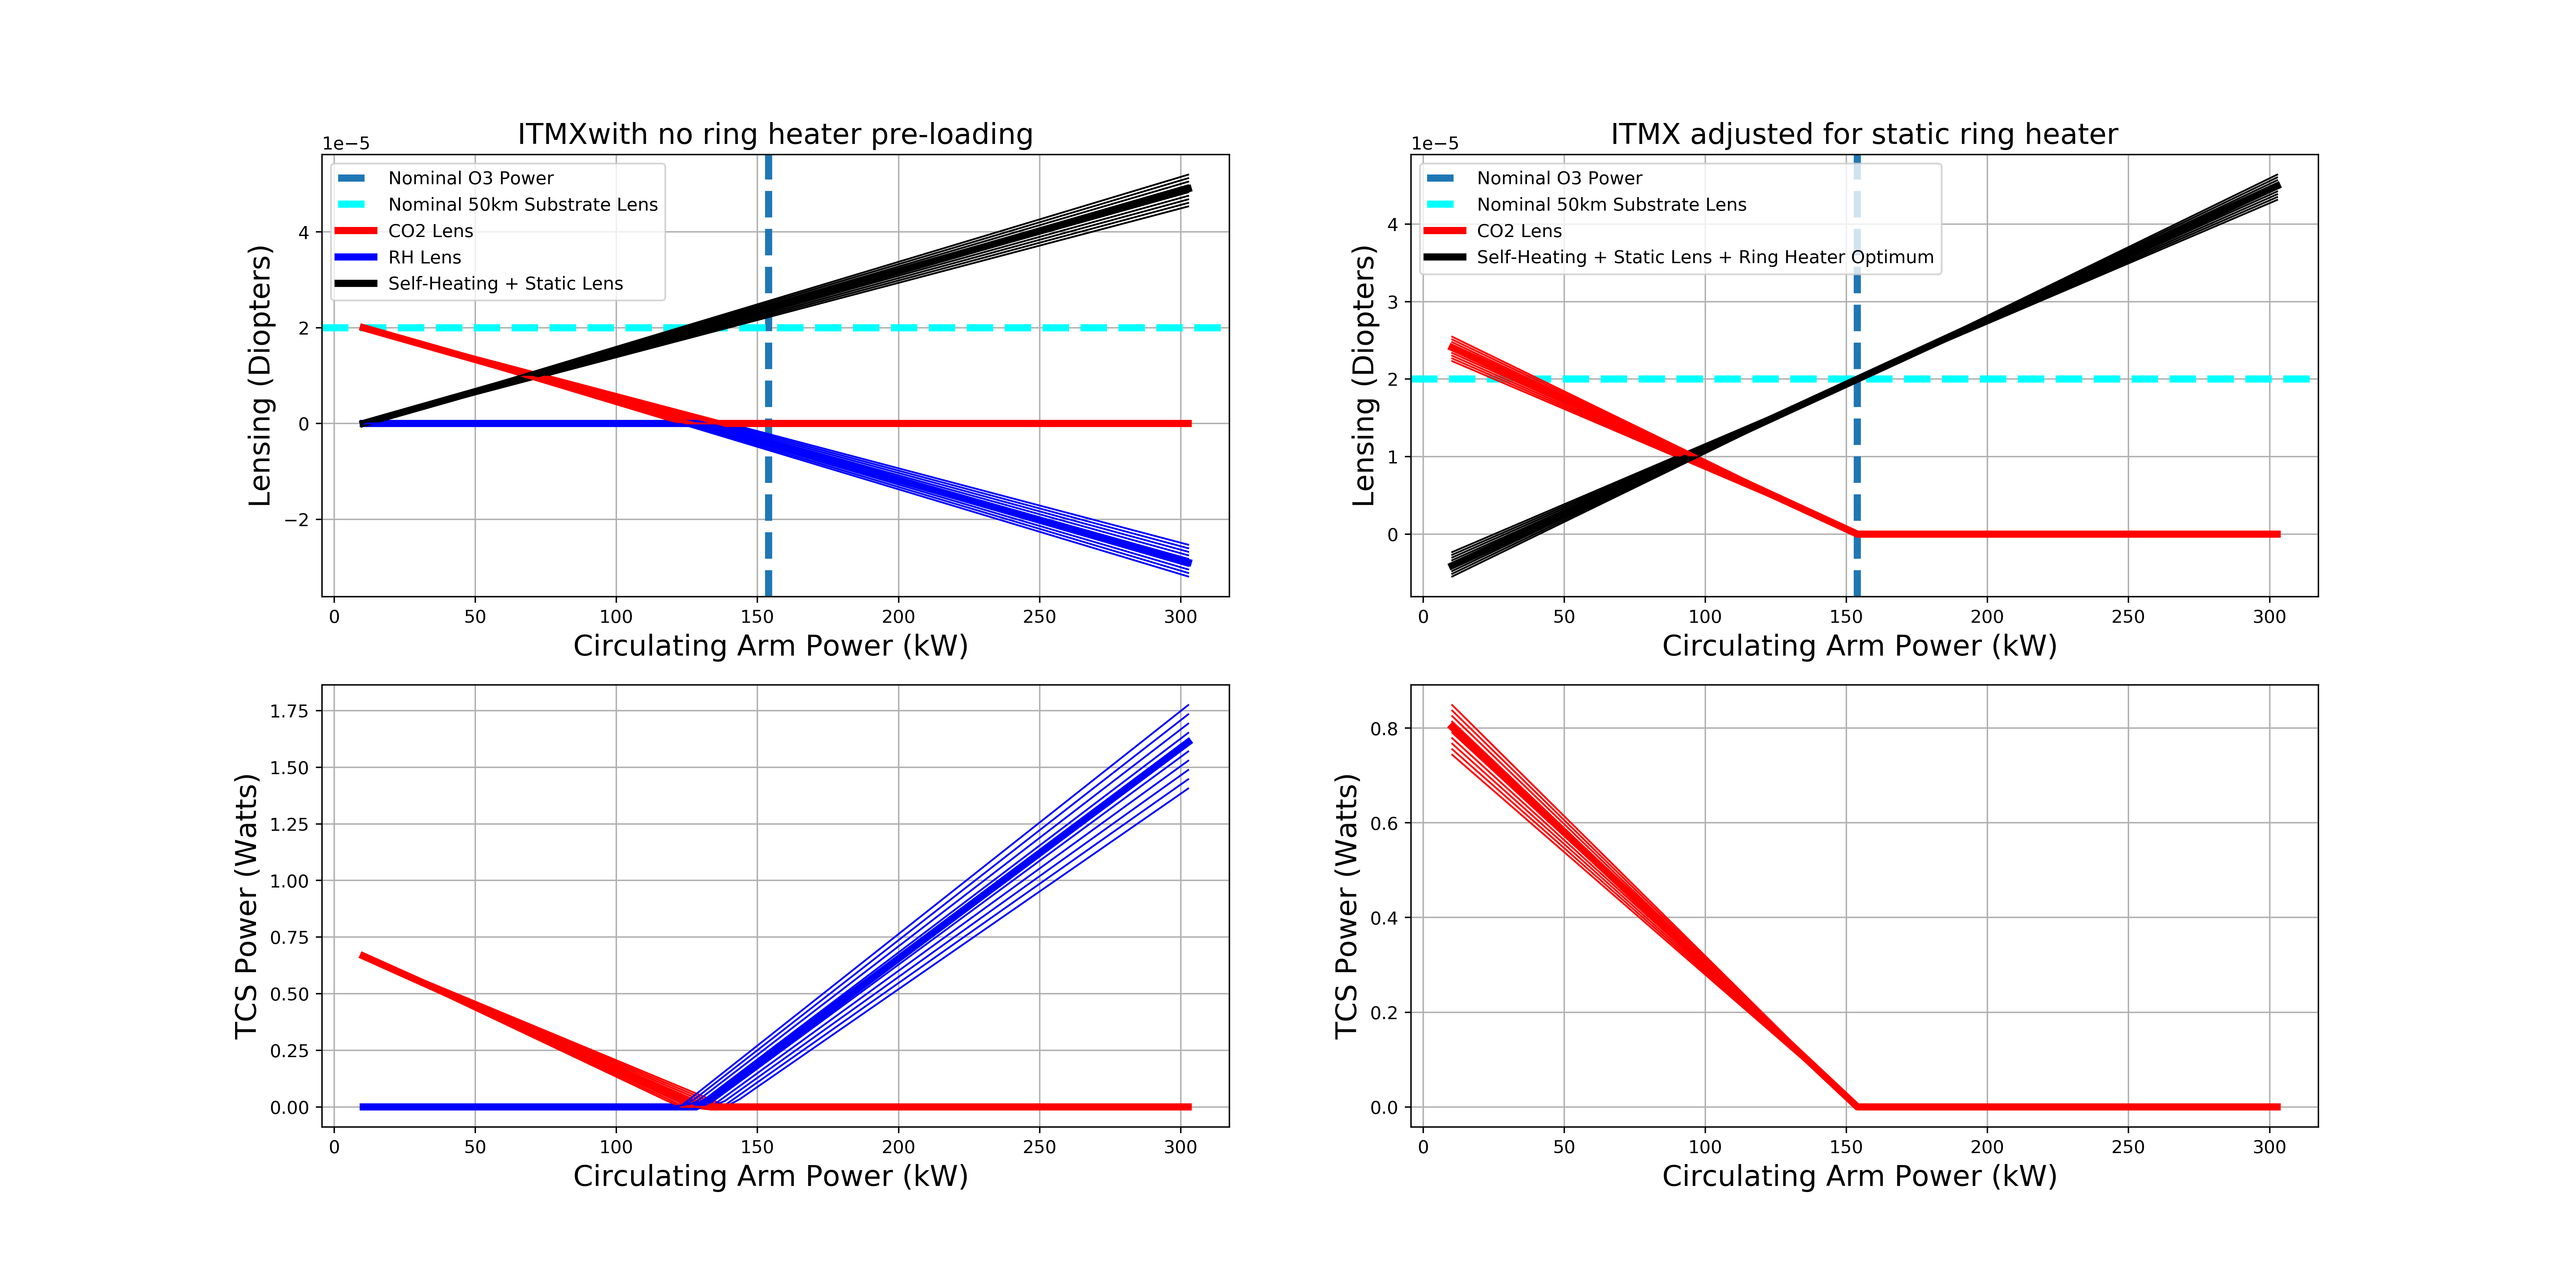
\includegraphics[width=1\textwidth]{ITMX_TCS_Settings.png}
            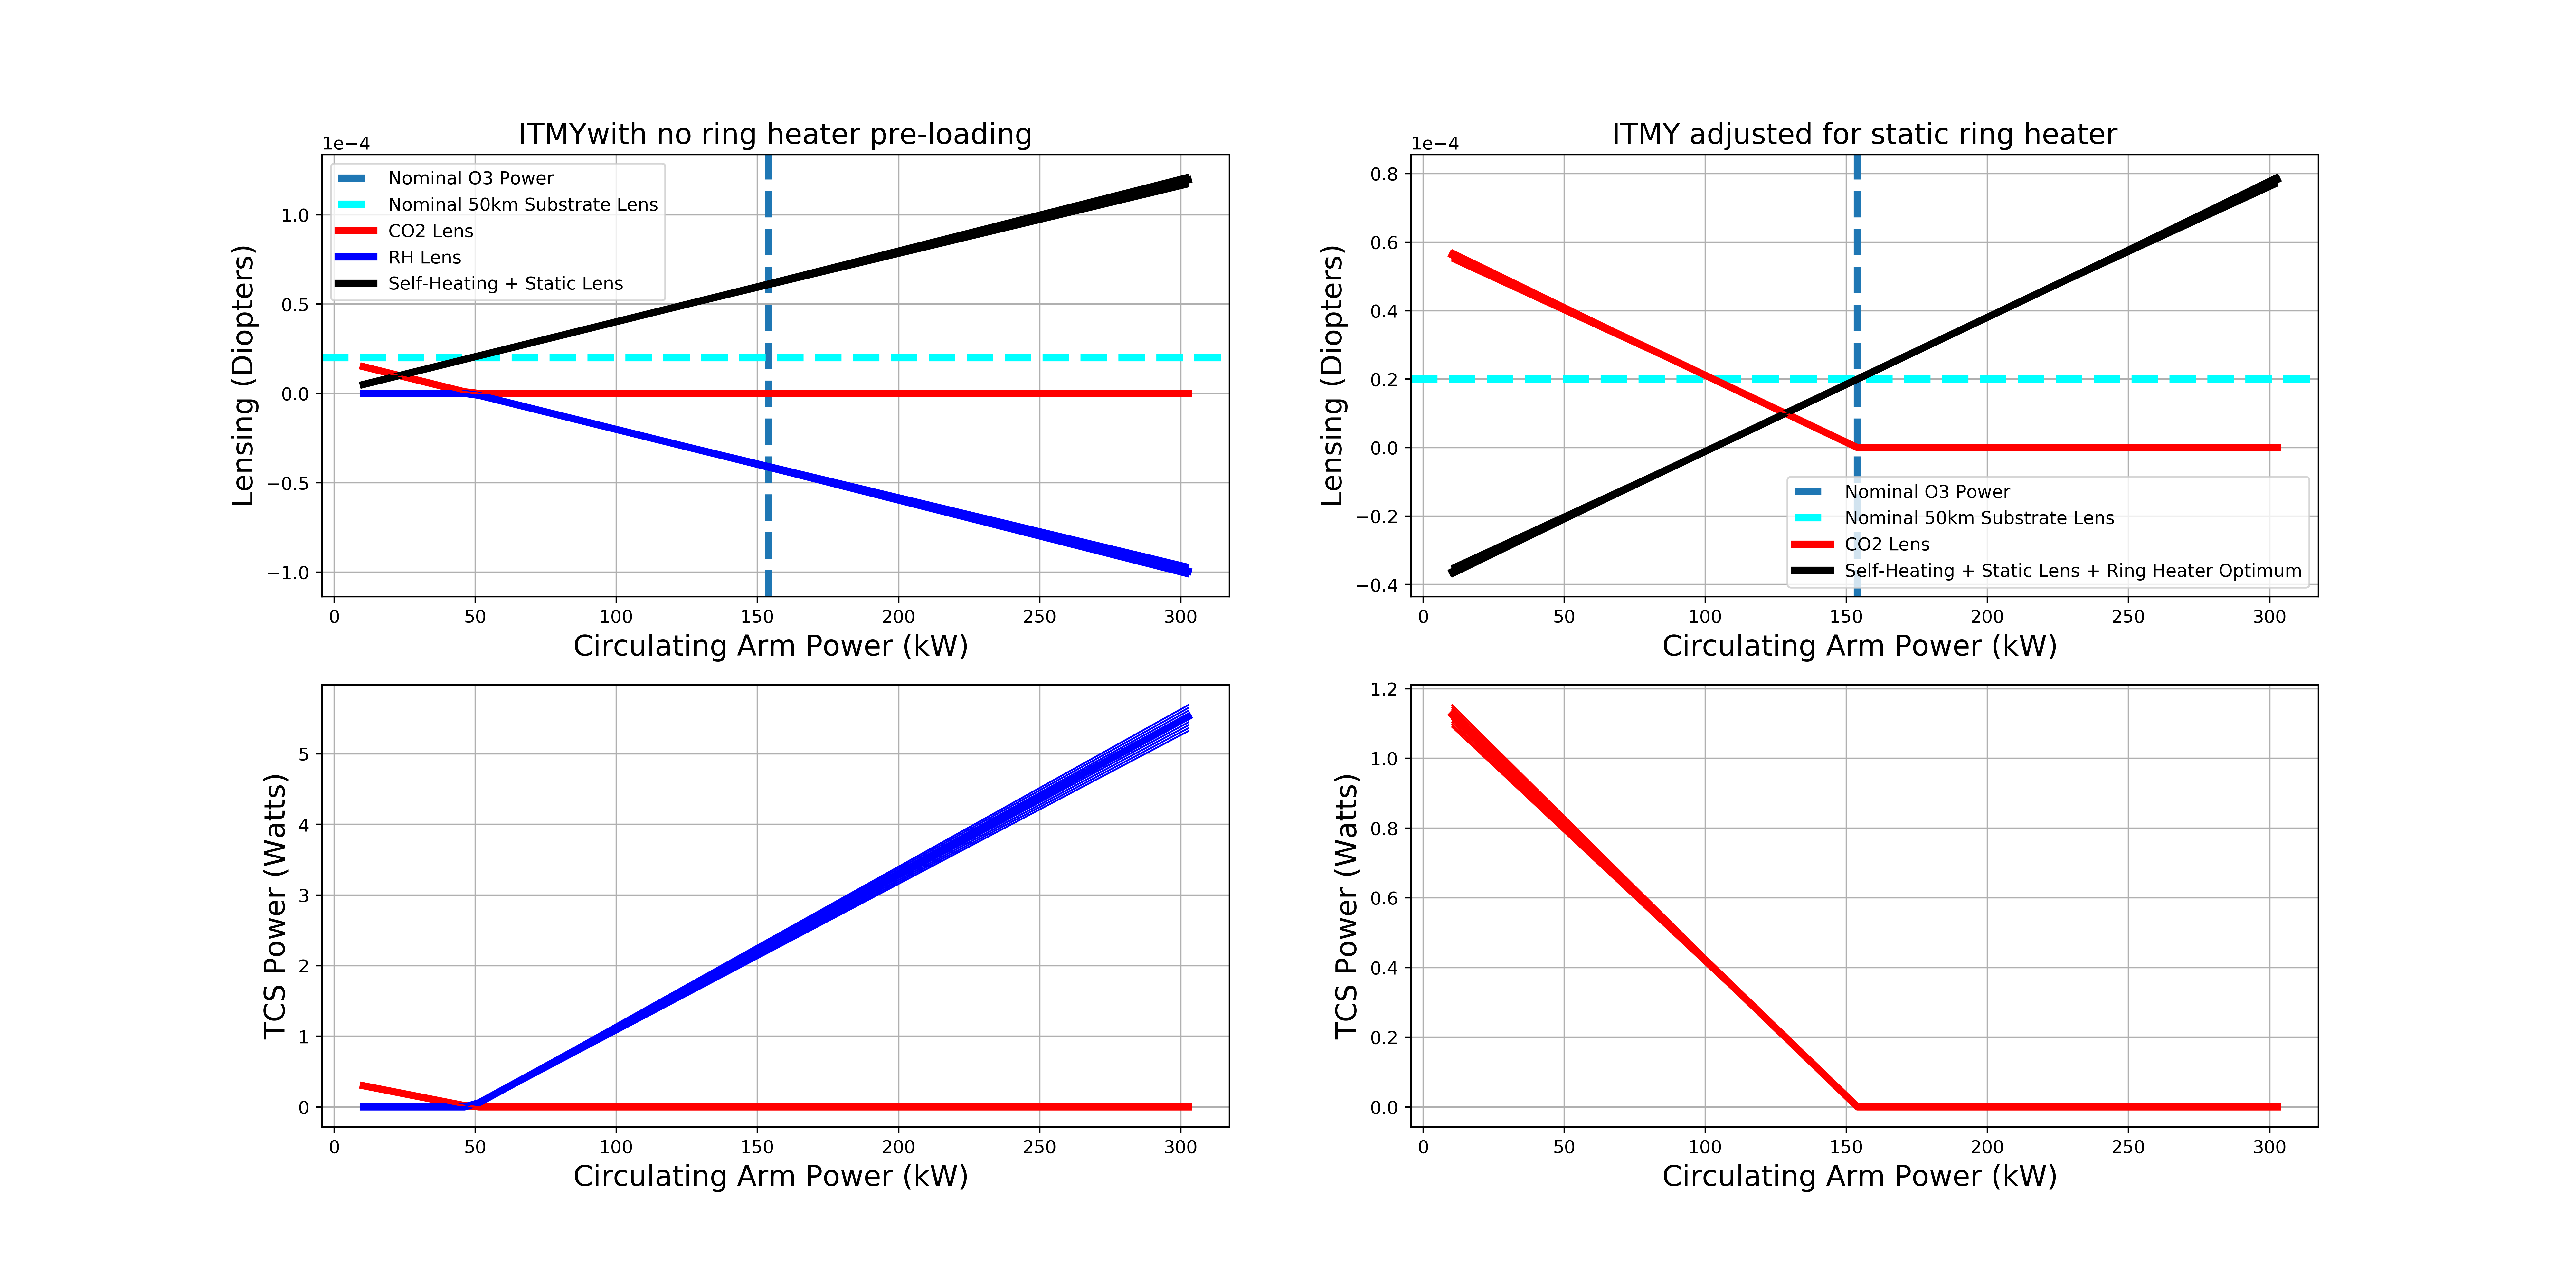
\includegraphics[width=1\textwidth]{ITMY_TCS_Settings.png}
            \caption{These plots assume that there are no high frequency spatial defects. PRG = 45, Arm gain = 228. Absorbed power for each test mass (in measurements) section. PC: Thomas Vo}
\end{figure}
    \item We separate TCS into two different states in the locking scheme while we attempt to achieve high power (assume we mean $\mathrm{P}_{\mathrm{in}} > 2 \mathrm{W}$): Preloading and High power operation. 

    \item Preloading
        \subitem The principle behind this state is to replicate the positive lens thermal distortions induced by a high power buildup within the interferometer arms and to properly compensate with the ring heaters to achieve an overall 50 km nominal lens. 
            \subsubitem Positive lens thermal distortions are replicated with CO2 lasers on the ITMX and ITMY compensation plates. 
        \subitem Allows for realistic commissioning of the interferometer controls in a "high power" thermal state.

    \item High power operation
        \subitem This state is achieved when increasing the input laser power (above 2 W) to a locked interferometer. 

\end{itemize}
